\documentclass[fontsize=11pt]{article}
\usepackage{amsmath}
\usepackage[utf8]{inputenc}
\usepackage[margin=0.75in]{geometry}
\usepackage{graphicx}
\usepackage{hyperref}

\everymath{\displaystyle}

\title{CSC110 Final Project: Your Anxiety During COVID-19}
\author{Fardin Faruk, Sharon Hsieh, Sinan Li, Jeffery Zhan}
\date{Tuesday, Dec 14, 2021}

\begin{document}
    \maketitle

    \section*{Introduction}
    Severe acute respiratory syndrome coronavirus 2 (SARS-CoV-2), commonly known for causing the illness COVID-19, spread wildly after its emergence in late 2019 (Britannica, T. Editors of Encyclopaedia, 2021).
    Following its discovery, society as we knew it was upended, and countries went into lockdown.
    Individuals were required to stay home to prevent the spread of the virus, restricting any socializing to very minimal interactions with others.
    Tested by working from home, unemployment, lack of social connections and many more challenges, many individuals found it challenging to adapt, making them especially vulnerable to mental health complications (World Health Organization, 2021).

    While COVID-19 has proven challenging to combat, Canada has put forth their best efforts to prevent the spread of the virus, becoming one of the top vaccinated countries in the world (Mathieu et al., 2021).
    Despite social regulations having been eased, many of the psychological effects linger.
    In fact, mental health has become such a prominent concern due to the pandemic that analysts at The National Institute of Mental Health now describe online therapy as essential (Prout, 2021).

    There is no doubt that the onset of the pandemic affected everyone differently — some found it easy to adjust, some struggled to do so, and many experienced some combination of the two — all for varying reasons.
    We have measured these differences quantitatively in order to answer the question: \textbf{what is the relationship between one’s identity and the degree to which COVID-19 has impacted their mental health?}

    Our research examines various traits that the subjects of the survey have, such as their education level, marital status, gender, and age, then compares their surveyed response to the pandemic alongside their traits and identities to determine a relationship between certain identity groups and the socio-psychological effects COVID-19 has had on them.
    From the results, we have ascertained which types of people are more susceptible to psychological issues due to the pandemic.
    We believe that this data can be applied to strengthen mental health resources and allow for more specialized and efficient care.

    \section*{Dataset Description}

    Dataset name: COVIDiSTRESS Global Survey Dataset \\
    Format: .csv \\
    Source: \url{https://doi.org/10.1038/s41597-020-00784-9} \\

	The COVIDiSTRESS Global Survey dataset on psychological and behavioural consequences of the COVID-19 outbreak (Yamada et al., 2020) is a survey which was organized by researchers in over 90 universities across the globe, investigating the mental health conditions and personal views surrounding COVID-19. It was conducted during the first major wave of the pandemic, and the responses of approximately 125,000 participants aged 18 and over, ranging across 42 countries, were recorded through this survey. The data is stored in a .csv file with each row containing information about a single person, including their gender, age, occupation status, marital status, and more. The file also includes each participant's responses to a broad range of questions posed on the survey about COVID-19. These questions range from questions about the individual’s support systems to questions about how they obtain information about COVID-19. \\

    In the csv file, each row contains information about a single surveyee and their responses to the survey, each of which is in a separate column. \\
    \\

    Columns used (starting count from column 0 which is just the initial numbering column):
    \begin{itemize}
        \item \texttt{Dem\_age [4]}
        \item \texttt{Dem\_gender [5]}
        \item \texttt{Dem\_edu [6]}
        \item \texttt{Dem\_employment [8]}
        \item \texttt{Country [9]}
        \item \texttt{Dem\_expat [10]}
        \item \texttt{Dem\_maritalstatus [12]}
        \item \texttt{Dem\_riskgroup [14]}
        \item \texttt{Dem\_islolation [15]}  (yes it's spelled like that)
        \item \texttt{Dem\_isolation\_adults [16]}
        \item \texttt{Dem\_isolation\_kids [17]}
    \end{itemize}

    Each of the above columns represents a specific identity group that a surveyee is a part of. The ones that we chose are the factors that we believe may influence the likeliness of an individual experiencing stress due to COVID-19 and its resulting effects. Among the categories that we chose to exclude, there was \texttt{Dem\_edu\_mom} (we did not think a person’s mother’s education was that significant), \texttt{Dem\_state} (we chose to categorize by country only), and \texttt{Dem\_dependents} (we made the decision to exclude this in favour of keeping \texttt{Dem\_isolation\_adults} and \texttt{Dem\_isolation\_kids}, which are similar but more straightforward).

    We also excluded the questions prefixed with ‘AD’ (\texttt{AD\_gain}, \texttt{AD\_loss}, \texttt{AD\_check}). These questions are meant to investigate the ‘framing effect’ and risk-averse choices, and we decided to exclude them because we did not believe they were relevant (Boyce, P., 2021).
    \begin{itemize}
        \item columns [21] to [48] (inclusive)
        \item columns [51] to [55] (inclusive)
        \item columns [70] to [72] (inclusive)
        \item column [80]
        \item column [82]
        \item columns [85] to [108] (inclusive)
        \item columns [110] to [135] (inclusive)
        \item columns [137] to [143] (inclusive)
    \end{itemize}

    The above are all survey questions that were measured on a Likert scale of 5, 6, or 11. We went through each survey question and decided whether or not it had any relevance towards indicating a person’s level of stress and anxiety. For this reason, we excluded questions such as to what extent the surveyee ‘appreciates art and aesthetics’. We also excluded any short-answer questions because those could not be quantified.

    \section*{Computational Overview}

    Our major data computations are performed in the file \texttt{data.py}.

    In the .csv (\texttt{COVIDiSTRESS June 17.csv}), each row represents the data of a single person and their answers to a set of survey questions.

    Within the function \texttt{read\_csv\_file}, we first initialize a list of dictionaries (\texttt{data\_processed\_so\_far}) in the function \texttt{initialize\_data\_list}, each dictionary being an ‘identity category’ (i.e. gender), and within it, the keys being specific ‘identity groups’ (i.e. male, female) and mapped to its own tuple; the first element of the tuple is the total number of participants that fit this group (according to their responses) and the second element is the total stress score of the entire population (which is the first element).

    Then we go through each row (person) and calculate their individual stress score (\texttt{stress\_score}) by going through their responses to the questions specified in the second part of our \textit{Data Description} section that specifically connect to how the surveyee feels about COVID-19 and various topics surrounding it. Their being measured on a Likert scale allows us to quantify their answers and numerically measure their feelings as well as worries about COVID-19.
    However, because of the varying range of the scales, we normalize each into the same range of values because weighing each question differently according to how relevant we felt it was proved to be out of the scope of our project. We do this by converting each scale into the same range of 0 to 4, inclusive, using an algorithm we formulated.
    However, we still needed to go through each question and decide whether higher values implied more stress on the surveyee's end or vice versa.

    With this, we take the sum of all their answers, \texttt{stress\_score} (with higher being more stressed), and add them to each dictionary in \texttt{data\_processed\_so\_far}. More specifically, the sum is added to the surveyee’s respective identity groups within the dictionaries (second element in the tuple), as well as +1 to the populations (first element in the tuple).

    The graphics user interface, GUI, was implemented using the \texttt{PyQt5} module. All of the work related to the look of the user interface and the user interaction logic was implemented in the \texttt{MainWindow} class in \texttt{ui.py}, a subclass of the \texttt{QMainWindow} class. It is the mainframe on which we put every other component -- widgets. The text displays, for example, \texttt{`Your Anxiety During COVID-19'}, or \texttt{`Country of Residence'}, were implemented using the \text{QLabel} class. The input fields consist of two types, with one being \texttt{QSpinBox} and the other being \texttt{QComboBox}. \texttt{QSpinBox} allows for numerical input, which we have set a reasonable range for each using the \texttt{QSpinBox.setRange} method provided. To get the current value, we used the \text{QSpinBox.value()} getter method. The \texttt{QComboBox}'s are drop-down menus, allowing the user to select from the drop-down list using a mouse or a keyboard. We can either get the selected text using the \texttt{QComboBox.getCurrentText} getter method, or get the index of the selected option using the \texttt{QComboBox.getCurrentIndex} method.

    The \textbf{user avatar}, a cartoon image generated based on the user's input, consists of layers of images. Every layer is a \texttt{QPixmap} instance -- a map of the pixels in the image. They are composed together using a \texttt{QPainter} element. Every layer is added by calling the \texttt{QPainter.drawImage()} method (Nemkin, 2010). Finally, to display the output, we place the pixmap onto a \texttt{QLabel} object using the \texttt{QLabel.setPixmap()} method. The \textbf{gauge} (Kibet, 2021) is implemented \texttt{gauge.py} as a subclass of the \texttt{QWidget} class -- the widget class in PyQt. The shapes, including the needle and the circles, are defined as the \texttt{QPolygon} or the \texttt{QPolygonF} class, with the first one using integer precision and the second one using floating-point precision. Essentially, they are the collection of 2-dimensional points -- an $x$ and a $y$ coordinate. The points are `drawn' using an instance of the \texttt{QPen} class. The \textbf{progress bar} is an \texttt{QProgressBar} object, and the `progress' is set using the \texttt{QProgressBar.setValue()} method.

    Using PyQt's signal and slot magnetism, the interface is capable of interacting with data in the backend. Using the \texttt{connect} method, we are able to connect signals -- events triggered automatically when a preset condition is met -- to specific functions. For example, when the user selects a new element from the drop-down menu for their `Gender' identity, the \texttt{QComboBox.currentIndexChanged} signal is emitted. By connecting this signal to updating the user's identity in the backend (as in line 298-299 in \texttt{ui.py}), and to updating the outputs like the gauge of the avatar (as line 316 in \texttt{ui.py}), any changes to the `Gender' identity would cause an immediate and automatic update to the outputs.

    The visualization of the processed data lies on the bottom left of the main window. This is implemented using the \texttt{pyqtgraph} library. Since every graph is a bar graph, the actual graph is defined as the \texttt{pyqtgraph.BarGraphItem} item (GeeksforGeeks, 2021). To set non-numerical axes labels (the identity), a \texttt{pyqthraph.AxisItem} object is used. To place the \texttt{BarGraphItem} onto the the main windos, it was placed into a \texttt{pyqtgraph.GraphicsLayoutWidget} object, which can then be placed into a \texttt{PyQt5.QtWidgets.QGridLayout} object.

    \section*{Instructions for obtaining datasets and running the program}
    Download the dataset: \url{https://osf.io/m5s8d/} \\
    Save the file \texttt{COVIDiSTRESS June 17.csv} in the \texttt{data} folder. \\

    Upon running \texttt{main.py}, the main user interface window and a pop-up window should appear. The pop-up window includes brief instructions on how to navigate the interface and can be closed once read. Start by entering one’s information using the input boxes and drop-down menus on the left. The character icon on the right will change based on different inputs. The graph on the bottom left of the interface displays the anxiety levels of different identities in a specific identity group. Use the drop-down menu above the graph to switch between different identity groups. On the right of the graph, the user’s likelihood of experiencing anxiety due to COVID-19 relative to the general population is displayed on a gauge. The user can also see their anxiety probability compared to specific identity groups using the drop-down menu on the far right of the window. This data is displayed using a progress bar. Finally, the user can find a textual summary of their data on the bottom right.

    \begin{center}
        This is what the program should like on a Windows computer:
    \end{center}
    \begin{center}
        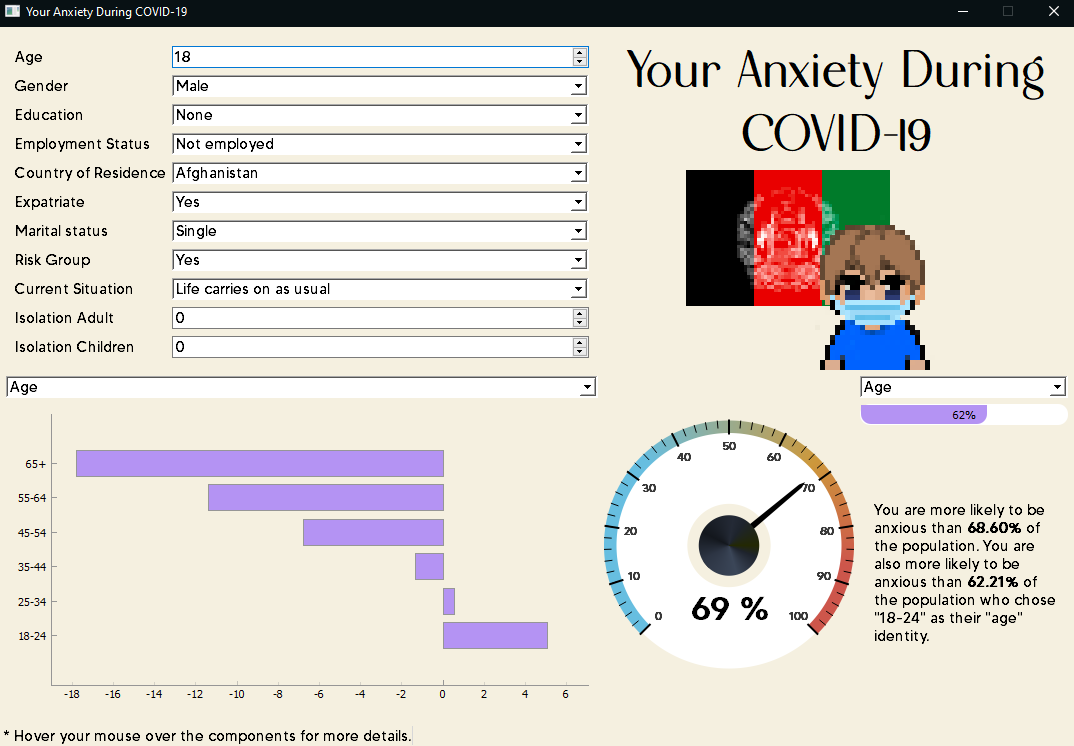
\includegraphics[scale=0.35]{img/example_screenshot}
    \end{center}

    \section*{Changes from the proposal to now}
    The feedback we received suggested that we implement regression in order to determine the most important factor in a person’s anxiety and stress levels. We experimented with the idea of this, taking a look at libraries such as SciKit and PyTorch. However, we decided that implementing regression would be beyond the scope of our project and most likely unfeasible with the time constraints.

    Case studies in the final report were suggested as well and we have implemented those, so you will find them in the next section.

    \section*{Discussion}
    \textbf{Research Question: What is the relationship between one’s identity and the degree to which COVID-19 has impacted their mental health?} \\
    In order to answer our research question, it was necessary for us to determine a scale with which we can measure one’s anxiety. Through the calculations and aggregation we did with the responses in the dataset, we were able to measure the degree in which COVID-19 may impact an individual in two ways: by measuring each survey question on a scale from 0 to 4 to tally up a general “anxiety score”, and by comparing this score to the rest of the population to find a relative percent chance of experiencing anxiety. Using these methods, we were able to see clear results indicating how having a single differing trait may cause two otherwise similar individuals to be impacted differently by COVID-19. For instance, we can see an anxiety increase of at least 8\% between someone who is employed and someone who is not employed. Direct examples similar to this can also be seen in the case studies below. In this sense, we were able to answer our research question. \\

    \textbf{Limitations Encountered} \\
    With the data processing, we found that, despite the .csv purportedly being ‘cleaned’ (it was placed in the ‘cleaned’ directory on the site), there were some issues with the dataset.

    First of all, there were some odd answers, especially in the countries column. Some answers had spelling mistakes, varied in capitalization, or were just complete nonsense. Other columns were inconsistent with their possible answers. For example, many columns had ‘Other/would rather not say’ as a possible response, but then one column had ‘Other \textbf{or} would rather not say’ which caused trouble with dictionary key-lookup later on. Finally, there were anomalies in the dataset where some surveyees responded to certain questions with absurd numbers, such as being in isolation with 110 adults, or 110 children (110 being the highest possible answer to these questions), which seemed… highly unlikely.

	Regarding the GUI, we ran into some trouble with \texttt{PyTA}. In \texttt{gauge.py}, we had two functions that override functions provided by \texttt{PyQt}. Thus, we were unable to change the name of these two functions (\texttt{resizeEvent} and \texttt{paintEvent}) despite these names not conforming to \texttt{PythonTA’s} naming conventions. We also encountered a \texttt{no-name-in-module} error where \texttt{PythonTA} was unable to find the \texttt{QColor} class from \texttt{PyQt5.QtGui} in the import statement. However, this class exists and was able to be implemented in our code with no errors. \\

    \textbf{Further Exploration} \\
    To explore this topic further, we can consider implementing regression into our data processing. Using regression to determine which factors are most significant in affecting one’s mental health could increase the accuracy of our results.

    In terms of the visual elements of the user interface, there is room for improvement. However
    We can take the project further by letting the user see the data of multiple identity groups combined. For example, the average anxiety scores different employment statuses in Canada only. Or, similarly, a Canadian man can compare their anxiety score to other Canadians that identify as male. \\

    \textbf{Case Studies} \\
    Just for reference, here is our supposed profiles as first-year university students in Canada, if we were also at low-risk and not in isolation:

    \begin{center}
        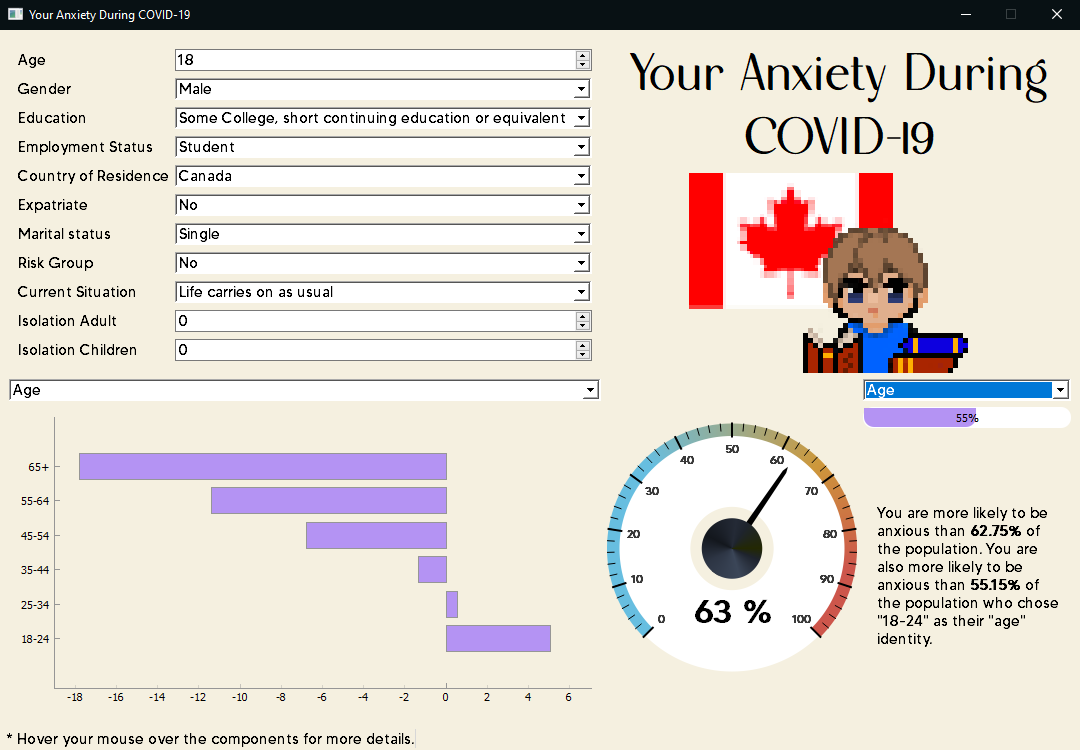
\includegraphics[scale=0.30]{img/male_student_screenshot}
        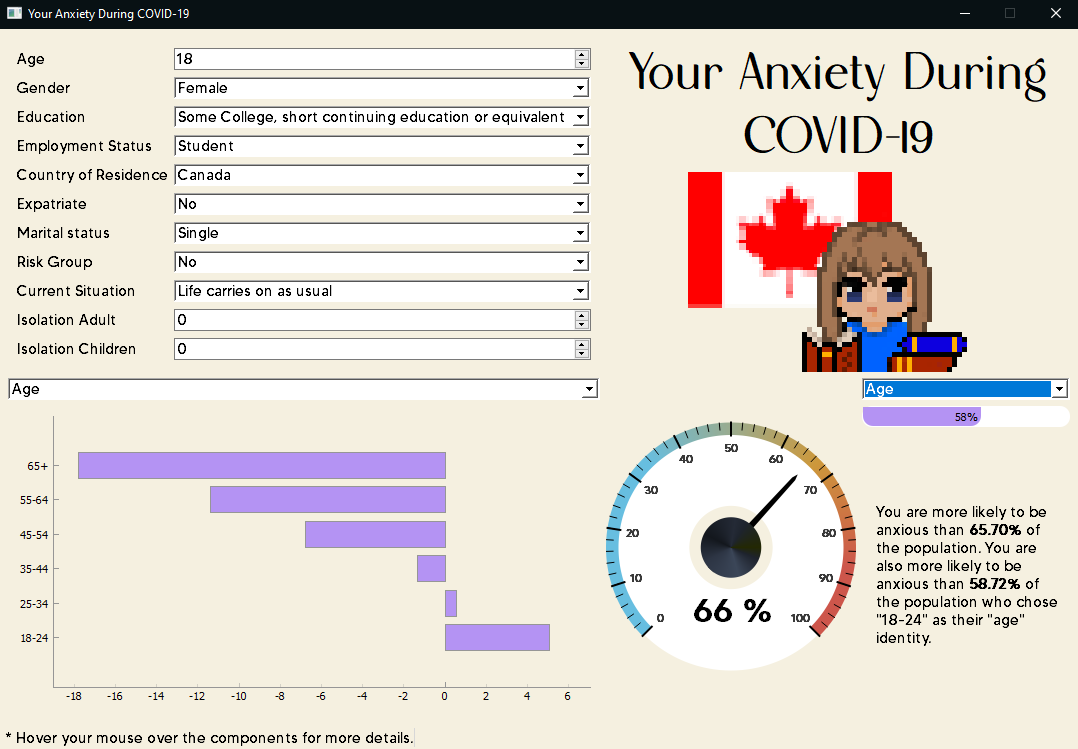
\includegraphics[scale=0.30]{img/female_student_screenshot}
    \end{center}

    Let’s contrast an unemployed man in his early 20’s to one in his 50s, retired with a PhD, and married.
    \begin{center}
        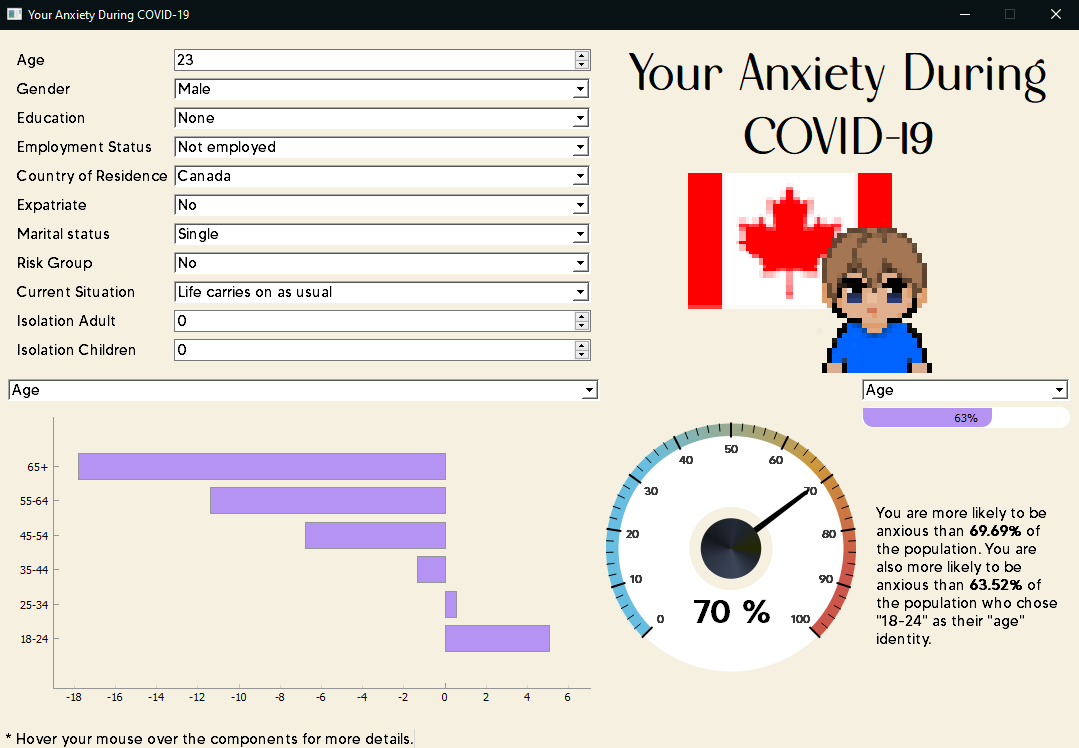
\includegraphics[scale=0.30]{img/casestudy_screenshot_1}
        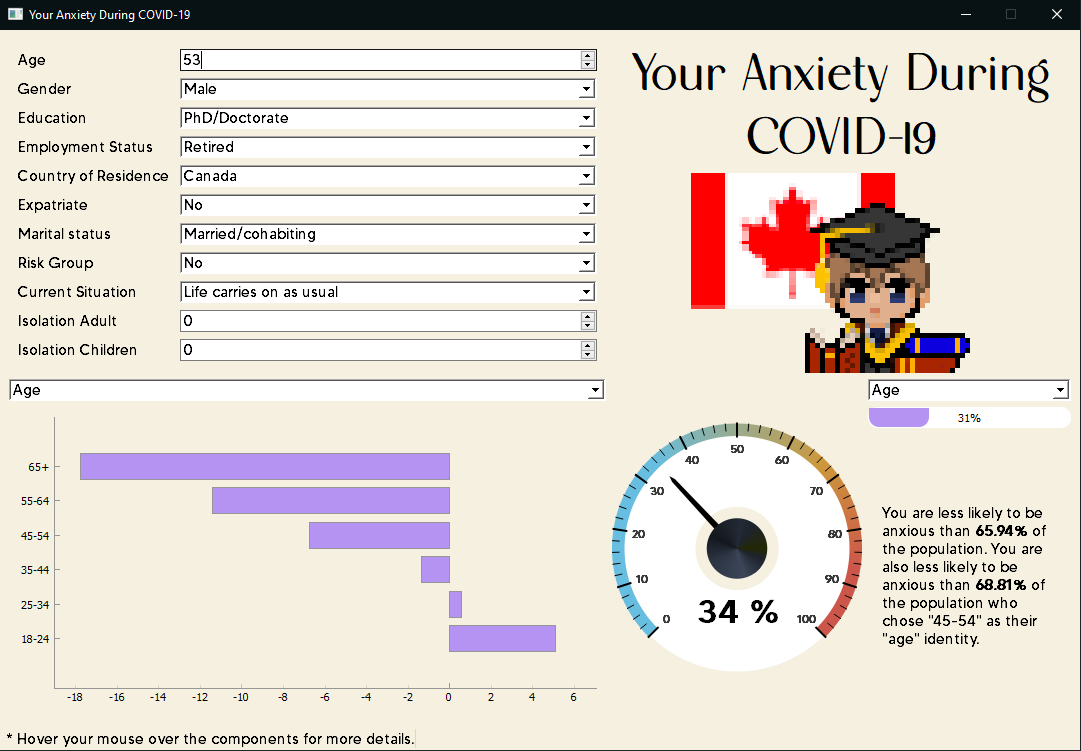
\includegraphics[scale=0.30]{img/casestudy_screenshot_2}
    \end{center}

    Here, we are looking at the extreme ends of the spectrum and there's a clear difference in their stress levels. The cause lies largely in the state of their education, employment status, and marital status: as one should expect, a person who is retired, has a PhD, and is married, should be more comfortable with his situation than a person in his early 20’s, who should expect to be either employed or still in school; he fulfills neither of those categories. Thus, he is more likely to experience anxiety considering the implications of his particular situation in the face of COVID-19, notorious for keeping unemployment rates low.
    
    Furthermore, if we adjust any of the person’s details, the gauge and percentage changes accordingly and within expectations: take the same retired person and consider if they were instead unemployed. They then rise to the upper echelons of the stressed, having a whopping 14\% higher likelihood for anxiety than the same person if retired. Again, employment status seems to be a critical factor in judging the probability of stress, which falls in line with expectations since in reality, employment status generally indicates a person’s financial stability. \\
    
    \textbf{Conclusion} \\
    In conclusion, we aggregated and filtered the data from the COVIDiSTRESS survey in order to discover the relationships between \texttt{stress\_score} and individuals’ identity groups. The final product of our findings is a GUI program that allows the user to input specific identities and receives a visual representation of their likelihood of anxiety, the average anxiety of the general population, and a comparison of the two. In doing so, we have found distinct relationships between one’s identity and the probability in which COVID-19 has impacted their mental health.

    \section*{References}

    \hangindent=0.7cm \noindent
    Boyce, P. (2021, October 16). \textit{Framing Effect Definition (5 Examples and 4 Types)}. BoyceWire.
    https://boycewire.co\\m/framing-effect-definition-and-examples/

    \hangindent=0.7cm \noindent
    Britannica, T. Editors of Encyclopaedia (2021, August 31). \textit{coronavirus}. \textit{Encyclopedia Britannica}.
    https://www.brita\\nnica.com/science/coronavirus-virus-group

    \hangindent=0.7cm \noindent
    Government of Canada. (2021).
    https://health-infobase.canada.ca/covid-19/epidemiological-summary-covid-19-cases.html

    \hangindent=0.7cm \noindent
    Kibet. K. (2021). \textit{QT-PyQt-PySide-Custom-Widgets} [Source code].
    https://github.com/KhamisiKibet/QT-PyQt-PySide-Custom-Widgets

    \hangindent=0.7cm \noindent
    luddek. (2015, August 14). \textit{Show string values on x-axis in pyqtgraph} Stack Overflow.
    https://stackoverflow.com/a/3\\2008832

    \hangindent=0.7cm \noindent
    Mathieu, E., Ritchie, H., Ortiz-Ospina, E., Roser, M., Hasell, J., Appel, C., Giattino, C., \& Rodés-Guirao, L. (2021). A global database of COVID-19 vaccinations. \textit{Nature Human Behaviour}, \textit{5}(7), 947-953. \\
    https://doi.org/10.1038/s41562-021-01122-8

    \hangindent=0.7cm \noindent
    Nemkin, N. (2010, December 7). \textit{How to add an image on the top of another image?} Stack Overflow.
    https://stackover\\flow.com/a/4379632

    \hangindent=0.7cm \noindent
    Prout, T. (2021, July 8). The importance of mental health during a pandemic. \textit{National University}.
    https://www.nu.e\\du/resources/the-importance-of-mental-health-during-a-pandemic/

    \hangindent=0.7cm \noindent
    pyqtgraph. (2021). \textit{PyQtGraph} (version 0.12.3) [Computer software].
    https://www.pyqtgraph.org/

    \hangindent=0.7cm \noindent
    rakshitarora. (2021, 05 May). \textit{PyQtGraph – Bar Graph} GeeksforGeeks.
    https://www.geeksforgeeks.org/pyqtgraph-bar-graph/

    \hangindent=0.7cm \noindent
    Riverbank Computing Limited. (2021). \textit{PyQt5} (Version 5.15.6) [Computer software].
    https://pypi.org/project/PyQt5/

    \hangindent=0.7cm \noindent
    World Health Organization. (2021). \textit{\#HealthyAtHome - Mental health}.
    https://www.who.int/campaigns/connecting-the-world-to-combat-coronavirus/healthyathome/healthyathome---mental-health

    \hangindent=0.7cm \noindent
    Yamada, Y., Ćepulić, D.-B., Coll-Martín, T., Debove, S., Gautreau, G., Han, H., Rasmussen, J., Tran, T. P., Travaglino, G. A., Blackburn, A. M., Boullu, L., Bujić, M., Byrne, G., Caniëls, M. C. J., Flis, I., Kowal, M., Rachev, N. R., Reynoso-Alcántara, V., Zerhouni, O. … Consortium, C. O. G. S. (2021). COVIDiSTRESS Global Survey dataset on psychological and behavioural consequences of the COVID-19 outbreak. \textit{Scientific Data}, \textit{8}(1), 3.
    https://doi.org/10.1038/s41597-020-00784-9

\end{document}
